\documentclass[11pt,a4paper]{report}
\usepackage[textwidth=37em,vmargin=30mm]{geometry}
\usepackage{calc,xunicode,amsmath,amssymb,paralist,enumitem,tabu,booktabs,datetime2,xeCJK,xeCJKfntef,listings}
\usepackage{tocloft,fancyhdr,tcolorbox,xcolor,graphicx,eso-pic,xltxtra,xelatexemoji}

\newcommand{\envyear}[0]{2025}
\newcommand{\envdatestr}[0]{2025-07-04}
\newcommand{\envfinaldir}[0]{webdb/2025/20250704/final}

\usepackage[hidelinks]{hyperref}
\hypersetup{
    colorlinks=false,
    pdfpagemode=FullScreen,
    pdftitle={Web Digest - \envdatestr}
}

\setlength{\cftbeforechapskip}{10pt}
\renewcommand{\cftchapfont}{\rmfamily\bfseries\large\raggedright}
\setlength{\cftbeforesecskip}{2pt}
\renewcommand{\cftsecfont}{\sffamily\small\raggedright}

\setdefaultleftmargin{2em}{2em}{1em}{1em}{1em}{1em}

\usepackage{xeCJK,xeCJKfntef}
\xeCJKsetup{PunctStyle=plain,RubberPunctSkip=false,CJKglue=\strut\hskip 0pt plus 0.1em minus 0.05em,CJKecglue=\strut\hskip 0.22em plus 0.2em}
\XeTeXlinebreaklocale "zh"
\XeTeXlinebreakskip = 0pt


\setmainfont{Brygada 1918}
\setromanfont{Brygada 1918}
\setsansfont{IBM Plex Sans}
\setmonofont{JetBrains Mono NL}
\setCJKmainfont{Noto Serif CJK SC}
\setCJKromanfont{Noto Serif CJK SC}
\setCJKsansfont{Noto Sans CJK SC}
\setCJKmonofont{Noto Sans CJK SC}

\setlength{\parindent}{0pt}
\setlength{\parskip}{8pt}
\linespread{1.15}

\lstset{
	basicstyle=\ttfamily\footnotesize,
	numbersep=5pt,
	backgroundcolor=\color{black!5},
	showspaces=false,
	showstringspaces=false,
	showtabs=false,
	tabsize=2,
	captionpos=b,
	breaklines=true,
	breakatwhitespace=true,
	breakautoindent=true,
	linewidth=\textwidth
}






\newcommand{\coverpic}[2]{
    % argv: itemurl, authorname
    Cover photo by #2~~(\href{#1}{#1})
}
\newcommand{\makeheader}[0]{
    \begin{titlepage}
        % \newgeometry{hmargin=15mm,tmargin=21mm,bmargin=12mm}
        \begin{center}
            
            \rmfamily\scshape
            \fontspec{BaskervilleF}
            \fontspec{Old Standard}
            \fontsize{59pt}{70pt}\selectfont
            WEB\hfill DIGEST
            
            \vfill
            % \vskip 30pt
            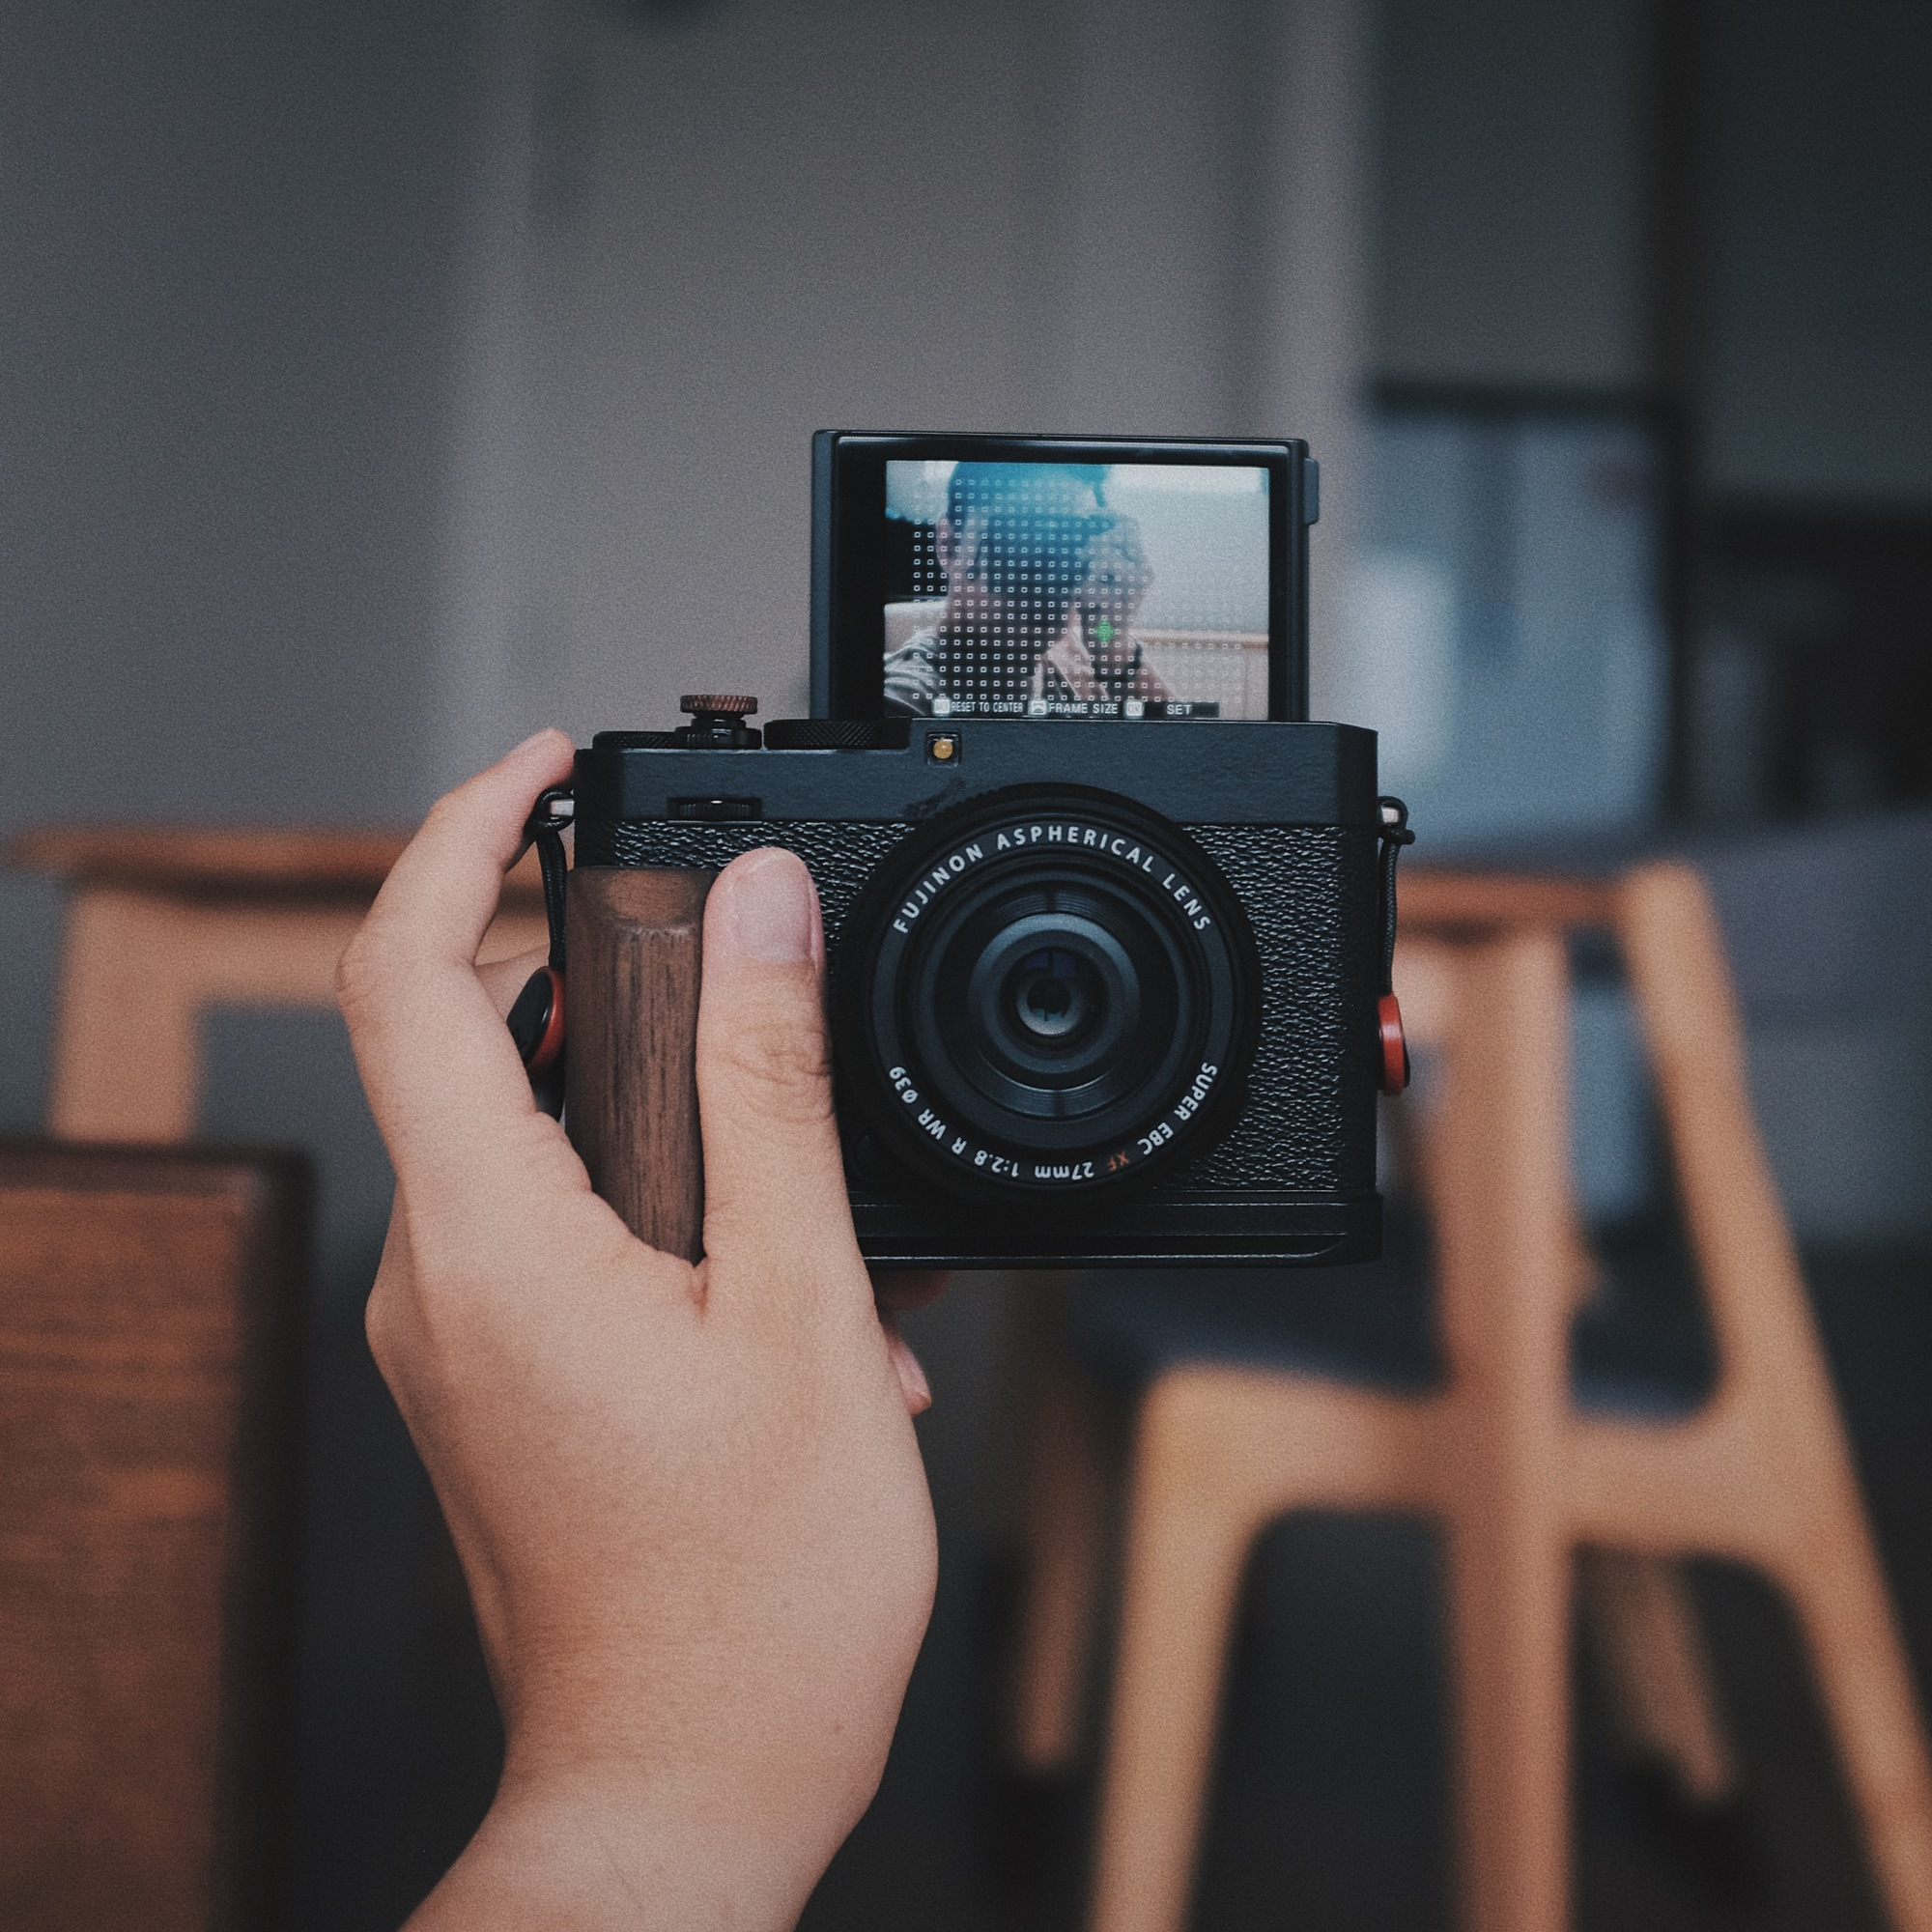
\includegraphics[width=\linewidth]{\envfinaldir/coverpic-prod.jpg}\par
            % \vskip 30pt
            \vfill

            \normalsize\rmfamily\scshape
            \copyright{} The Web Digest Project \hfill\large \envdatestr
        \end{center}
    \end{titlepage}
    % \restoregeometry
}
\newcommand{\simplehref}[1]{%
    \textcolor{blue!80!green}{\href{#1}{#1}}%
}
\renewcommand{\contentsname}{\center\Huge\sffamily\bfseries Contents\par\vskip 20pt}
\newcounter{ipartcounter}
\setcounter{ipartcounter}{0}
\newcommand{\ipart}[1]{
    % \vskip 20pt
    \clearpage
    \stepcounter{ipartcounter}
    \phantomsection
    \addcontentsline{toc}{chapter}{#1}
    % \begin{center}
    %     \Huge
    %     \sffamily\bfseries
    %     #1
    % \end{center}
    % \vskip 20pt plus 7pt
}
\newcounter{ichaptercounter}
\setcounter{ichaptercounter}{0}
\newcommand{\ichapter}[1]{
    % \vskip 20pt
    \clearpage
    \stepcounter{ichaptercounter}
    \phantomsection
    \addcontentsline{toc}{section}{\numberline{\arabic{ichaptercounter}}#1}
    \begin{center}
        \Huge
        \sffamily\bfseries
        #1
    \end{center}
    \vskip 20pt plus 7pt
}
\newcommand{\entrytitlefont}[1]{\subsection*{\raggedright\Large\sffamily\bfseries#1}}
\newcommand{\entryitemGeneric}[2]{
    % argv: title, url
    \parbox{\linewidth}{
        \entrytitlefont{#1}\par\vskip 5pt
        \footnotesize\ttfamily\mdseries
        \simplehref{#2}
    }\vskip 11pt plus 11pt minus 1pt
}
\newcommand{\entryitemGithub}[3]{
    % argv: title, url, desc
    \parbox{\linewidth}{
        \entrytitlefont{#1}\par\vskip 5pt
        \footnotesize\ttfamily\mdseries
        \simplehref{#2}\par\vskip 5pt
        \small\rmfamily\mdseries#3
    }\vskip 11pt plus 11pt minus 1pt
}
\newcommand{\entryitemAp}[3]{
    % argv: title, url, desc
    \parbox{\linewidth}{
        \entrytitlefont{#1}\par\vskip 5pt
        \footnotesize\ttfamily\mdseries
        \simplehref{#2}\par\vskip 5pt
        \small\rmfamily\mdseries#3
    }\vskip 11pt plus 11pt minus 1pt
}
\newcommand{\entryitemHackernews}[3]{
    % argv: title, hnurl, rawurl
    % \parbox{\linewidth}{
    %     \entrytitlefont{#1}\par\vskip 5pt
    %     \footnotesize\ttfamily\mdseries
    %     \simplehref{#3}\par
    %     \textcolor{black!50}{\href{#2}{#2}}
    % }\vskip 11pt plus 11pt minus 1pt
    \begin{minipage}{\linewidth}
            \entrytitlefont{#1}\par\vskip 5pt
            \footnotesize\ttfamily\mdseries
            \simplehref{#3}\par
            \textcolor{black!50}{\href{#2}{#2}}
    \end{minipage}\par\vskip 11pt plus 11pt minus 1pt
}







\begin{document}

\makeheader

\tableofcontents\clearpage




\ipart{Developers}
\ichapter{Hacker News}
\entryitemTwoLinks{Opening up `Zero-Knowledge Proof' technology}{https://news.ycombinator.com/item?id=44457390}{https://blog.google/technology/safety-security/opening-up-zero-knowledge-proof-technology-to-promote-privacy-in-age-assurance/}

\entryitemTwoLinks{Launch HN: K-Scale Labs (YC W24) – Open-Source Humanoid Robots}{https://news.ycombinator.com/item?id=44456904}{https://news.ycombinator.com/item?id=44456904}

\entryitemTwoLinks{AV1@Scale: Film Grain Synthesis, The Awakening}{https://news.ycombinator.com/item?id=44456779}{https://netflixtechblog.com/av1-scale-film-grain-synthesis-the-awakening-ee09cfdff40b}

\entryitemTwoLinks{Poor Man's Back End-as-a-Service (BaaS), Similar to Firebase/Supabase/Pocketbase}{https://news.ycombinator.com/item?id=44456135}{https://github.com/zserge/pennybase}

\entryitemTwoLinks{Flounder Mode – Kevin Kelly on a different way to do great work}{https://news.ycombinator.com/item?id=44455933}{https://joincolossus.com/article/flounder-mode/}

\entryitemTwoLinks{Introducing tmux-rs}{https://news.ycombinator.com/item?id=44455787}{https://richardscollin.github.io/tmux-rs/}

\entryitemTwoLinks{Peasant Railgun}{https://news.ycombinator.com/item?id=44455222}{https://knightsdigest.com/what-exactly-is-the-peasant-railgun-in-dd-5e/}

\entryitemTwoLinks{Where is my von Braun wheel?}{https://news.ycombinator.com/item?id=44455022}{https://angadh.com/wherevonbraunwheel}

\entryitemTwoLinks{Show HN: HomeBrew HN – Generate personal context for content ranking}{https://news.ycombinator.com/item?id=44454305}{https://www.hackernews.coffee/}

\entryitemTwoLinks{The uv build back end is now stable}{https://news.ycombinator.com/item?id=44454061}{https://docs.astral.sh/uv/concepts/build-backend/}

\entryitemTwoLinks{Tools: Code Is All You Need}{https://news.ycombinator.com/item?id=44453688}{https://lucumr.pocoo.org/2025/7/3/tools/}

\entryitemTwoLinks{I scanned all of GitHub's "oops commits" for leaked secrets}{https://news.ycombinator.com/item?id=44452317}{https://trufflesecurity.com/blog/guest-post-how-i-scanned-all-of-github-s-oops-commits-for-leaked-secrets}

\entryitemTwoLinks{Astronomers discover 3I/ATLAS – Third interstellar object to visit Solar System}{https://news.ycombinator.com/item?id=44451329}{https://www.abc.net.au/news/science/2025-07-03/3i-atlas-a11pl3z-interstellar-object-in-our-solar-system/105489180}

\entryitemTwoLinks{Trans-Taiga Road (2004)}{https://news.ycombinator.com/item?id=44450575}{https://www.jamesbayroad.com/ttr/index.html}

\entryitemTwoLinks{Whole-genome ancestry of an Old Kingdom Egyptian}{https://news.ycombinator.com/item?id=44450304}{https://www.nature.com/articles/s41586-025-09195-5}

\entryitemTwoLinks{Gmailtail – Command-line tool to monitor Gmail messages and output them as JSON}{https://news.ycombinator.com/item?id=44450182}{https://github.com/c4pt0r/gmailtail}

\entryitemTwoLinks{What to build instead of AI agents}{https://news.ycombinator.com/item?id=44450160}{https://decodingml.substack.com/p/stop-building-ai-agents}

\entryitemTwoLinks{American science to soon face its largest brain drain in history}{https://news.ycombinator.com/item?id=44449614}{https://bigthink.com/starts-with-a-bang/american-science-brain-drain/}

\entryitemTwoLinks{TikTok is being flooded with racist AI videos generated by Google's Veo 3}{https://news.ycombinator.com/item?id=44449486}{https://arstechnica.com/ai/2025/07/racist-ai-videos-created-with-google-veo-3-are-proliferating-on-tiktok/}

\entryitemTwoLinks{Websites hosting major US climate reports taken down}{https://news.ycombinator.com/item?id=44448868}{https://apnews.com/article/climate-change-national-assessment-nasa-white-house-057cec699caef90832d8b10f21a6ffe8}


\ipart{Developers~~~~(zh-Hans)}
\ichapter{Solidot}
\entryitemGeneric{\hskip 0pt{}海绵结构材料借助太阳热能去除海水中的盐分 }{https://www.solidot.org/story?sid=81717}

\entryitemGeneric{\hskip 0pt{}系外行星引发恒星释放耀斑}{https://www.solidot.org/story?sid=81716}

\entryitemGeneric{\hskip 0pt{}男女对婴儿晚上哭泣声音的反应差别不大}{https://www.solidot.org/story?sid=81715}

\entryitemGeneric{\hskip 0pt{}美国年轻人减少了游戏开支}{https://www.solidot.org/story?sid=81714}

\entryitemGeneric{\hskip 0pt{}TikTok 涌现大量 Google Veo 3 生成的种族主义视频}{https://www.solidot.org/story?sid=81713}

\entryitemGeneric{\hskip 0pt{}微软裁员约九千人,游戏业务深受影响}{https://www.solidot.org/story?sid=81712}

\entryitemGeneric{\hskip 0pt{}天文学家可能发现了已知第三个星际天体}{https://www.solidot.org/story?sid=81711}

\entryitemGeneric{\hskip 0pt{}测试 Firefox 120 到 Firefox 141 在 Linux 下的性能}{https://www.solidot.org/story?sid=81710}

\entryitemGeneric{\hskip 0pt{}任天堂有意锁定 Switch 2 的 USB-C 端口阻止第三方扩展坞}{https://www.solidot.org/story?sid=81709}

\entryitemGeneric{\hskip 0pt{}Copyleft-next 项目重新启动}{https://www.solidot.org/story?sid=81708}

\entryitemGeneric{\hskip 0pt{}西北工业大学成功试飞飞天二号高超音速飞行器}{https://www.solidot.org/story?sid=81707}

\entryitemGeneric{\hskip 0pt{}顶级 AI 工程师的薪水最高超过千万美元}{https://www.solidot.org/story?sid=81706}

\entryitemGeneric{\hskip 0pt{}数据不支持左撇子更具创造力的观点}{https://www.solidot.org/story?sid=81705}

\entryitemGeneric{\hskip 0pt{}OsmAnd 地图应用项目诞生 15 周年}{https://www.solidot.org/story?sid=81704}

\entryitemGeneric{\hskip 0pt{}华为发布了使用昇腾 NPU 训练的开放权重模型}{https://www.solidot.org/story?sid=81703}

\entryitemGeneric{\hskip 0pt{}首批美国科学难民抵达法国}{https://www.solidot.org/story?sid=81702}

\entryitemGeneric{\hskip 0pt{}炎症衰老可能是工业化生活方式的产物}{https://www.solidot.org/story?sid=81701}

\entryitemGeneric{\hskip 0pt{}GNU Health Hospital Information System 5.0 释出}{https://www.solidot.org/story?sid=81700}

\entryitemGeneric{\hskip 0pt{}RisingAttacK 攻击让 AI ``看到''你想让它看到的内容}{https://www.solidot.org/story?sid=81699}

\entryitemGeneric{\hskip 0pt{}美国卫生部称《自然》是垃圾科学,全面取消订阅《自然》期刊}{https://www.solidot.org/story?sid=81698}\ichapter{V2EX}
\entryitemGeneric{\hskip 0pt{}[分享发现] [分享]-能够查询 I2C 设备的网站}{https://www.v2ex.com/t/1142899}

\entryitemGeneric{\hskip 0pt{}[问与答] IOS 抓包有的抓不到是什么原因,怎么样才能抓包调试呢?}{https://www.v2ex.com/t/1142898}

\entryitemGeneric{\hskip 0pt{}[问与答] 请问各位有什么认证好考的。}{https://www.v2ex.com/t/1142897}

\entryitemGeneric{\hskip 0pt{}[问与答] 把 案情 基本信息描述一遍 利用 ai 可以给我一个近似的裁判文书吗? do it}{https://www.v2ex.com/t/1142892}

\entryitemGeneric{\hskip 0pt{}[问与答] AI 最终会不会取代普通程序员呢?}{https://www.v2ex.com/t/1142891}

\entryitemGeneric{\hskip 0pt{}[程序员] 大家都阿里开源的项目怎么看}{https://www.v2ex.com/t/1142889}

\entryitemGeneric{\hskip 0pt{}[求职] [广州]连续创业者,技术开发老人求职(二)}{https://www.v2ex.com/t/1142888}

\entryitemGeneric{\hskip 0pt{}[程序员] 感觉差不多也到职业生涯末期了}{https://www.v2ex.com/t/1142886}

\entryitemGeneric{\hskip 0pt{}[问与答] 请推荐一个用于 Office 文档类文件的版本控制软件要求简单好用,可以随时双击查看旧版本文件无需下载。}{https://www.v2ex.com/t/1142885}

\entryitemGeneric{\hskip 0pt{}[问与答] 哪里有公众号互阅互赞这种群或者平台?}{https://www.v2ex.com/t/1142883}

\entryitemGeneric{\hskip 0pt{}[程序员] 目前哪个大模型适合本地部署用来纯翻译?}{https://www.v2ex.com/t/1142882}

\entryitemGeneric{\hskip 0pt{}[宽带症候群] 南京联通体验如何?}{https://www.v2ex.com/t/1142881}

\entryitemGeneric{\hskip 0pt{}[问与答] pbt 键帽打油有什么解决办法?}{https://www.v2ex.com/t/1142880}

\entryitemGeneric{\hskip 0pt{}[问与答] 发现一个很奇葩的问题,同一个直播 app 在 ios 和安卓的客户端内播放速度不一样}{https://www.v2ex.com/t/1142879}

\entryitemGeneric{\hskip 0pt{}[Lightroom] 求教!为什么 Lightroom 没有很好的自动化流程?}{https://www.v2ex.com/t/1142878}

\entryitemGeneric{\hskip 0pt{}[程序员] 国内服务器有什么方便的从 git 仓库指定分支同步部署前后端代码简单 CI/CD 方案吗?}{https://www.v2ex.com/t/1142876}

\entryitemGeneric{\hskip 0pt{}[问与答] plc 好不好玩?单片机有点玩腻了}{https://www.v2ex.com/t/1142875}

\entryitemGeneric{\hskip 0pt{}[Cursor] cursor 限流,大概 3 个小时重置}{https://www.v2ex.com/t/1142873}

\entryitemGeneric{\hskip 0pt{}[分享创造] 闲着没事做了个医保药品目录查询系统,欢迎围观}{https://www.v2ex.com/t/1142870}

\entryitemGeneric{\hskip 0pt{}[云计算] 关于用 terraform 管理腾讯云上的资源的问题}{https://www.v2ex.com/t/1142869}

\entryitemGeneric{\hskip 0pt{}[推广] 程序员为什么要出海赚美刀?}{https://www.v2ex.com/t/1142868}

\entryitemGeneric{\hskip 0pt{}[酷工作] [招聘-远程办公] 金融产品经理}{https://www.v2ex.com/t/1142867}

\entryitemGeneric{\hskip 0pt{}[分享创造] 🎁 华为 700 元云资源券获取指南(保姆级教程)}{https://www.v2ex.com/t/1142866}

\entryitemGeneric{\hskip 0pt{}[酷工作] New/Hot Jobs: 低延迟量化交易开发工程师(可提供 EP)}{https://www.v2ex.com/t/1142862}

\entryitemGeneric{\hskip 0pt{}[Apple] 京东 m4pro 24G 512 10G 以太网 macmini 史低}{https://www.v2ex.com/t/1142860}

\entryitemGeneric{\hskip 0pt{}[Mac mini] MacOS 27 寸 4K 显示器该用哪个分辨率?}{https://www.v2ex.com/t/1142859}

\entryitemGeneric{\hskip 0pt{}[问与答] 咸鱼出 switch 游戏机现在感觉被骗了 掉包我的内存卡}{https://www.v2ex.com/t/1142858}

\entryitemGeneric{\hskip 0pt{}[推广] 搞了个 Sprunki 游戏站. 虽然热度已经过去了,但是从追赶和模仿开始.}{https://www.v2ex.com/t/1142857}

\entryitemGeneric{\hskip 0pt{}[问与答] 国内创业贸易类小公司,要不要坚持}{https://www.v2ex.com/t/1142856}

\entryitemGeneric{\hskip 0pt{}[酷工作] 远程高级 PHP 开发工程师}{https://www.v2ex.com/t/1142855}

\entryitemGeneric{\hskip 0pt{}[程序员] minio 替代, rustfs 终于开源了}{https://www.v2ex.com/t/1142853}

\entryitemGeneric{\hskip 0pt{}[程序员] 请问有必要用专门的消息队列吗? all in sqldb 是否可行?}{https://www.v2ex.com/t/1142852}

\entryitemGeneric{\hskip 0pt{}[程序员] [请教大家] 大家好,最近不好找工作。我想尝试组个外包团队自己干,接点价格比较高的定制化项目。请问大家有没有方式能找到客户呀?上海地区}{https://www.v2ex.com/t/1142851}

\entryitemGeneric{\hskip 0pt{}[问与答] 电车开了 3 年 发现省钱不省油}{https://www.v2ex.com/t/1142850}

\entryitemGeneric{\hskip 0pt{}[VXNA] 申请收录个人博客: Tomyail 的记忆现场}{https://www.v2ex.com/t/1142849}

\entryitemGeneric{\hskip 0pt{}[程序员] 一个工作一年的后端码农,最佳情况下应该掌握哪些专业知识}{https://www.v2ex.com/t/1142848}

\entryitemGeneric{\hskip 0pt{}[程序员] py 程序你们喜欢一个 config 传来传去吗}{https://www.v2ex.com/t/1142846}

\entryitemGeneric{\hskip 0pt{}[反馈] 我的账号是被降权了吗,为什么我发布的内容不会像之前一样在推荐流的前面了}{https://www.v2ex.com/t/1142843}

\entryitemGeneric{\hskip 0pt{}[游戏] 分享一下开发的最无厘头的 AI PVP 游戏「脑洞大乱斗」}{https://www.v2ex.com/t/1142842}

\entryitemGeneric{\hskip 0pt{}[职场话题] 海外 APP 开发交流群,欢迎加入}{https://www.v2ex.com/t/1142841}

\entryitemGeneric{\hskip 0pt{}[酷工作] 公司投标需要协助准备技术资料,找一位硕士+ 5 年经验的软件同行}{https://www.v2ex.com/t/1142840}

\entryitemGeneric{\hskip 0pt{}[京东] 京东购买的安克充电宝在召唤范围内,无法在京东申请售后。}{https://www.v2ex.com/t/1142839}

\entryitemGeneric{\hskip 0pt{}[酷工作] 今年广州 boss 上的招聘信息,为什么 10 家有 9 家都是语音房?}{https://www.v2ex.com/t/1142838}

\entryitemGeneric{\hskip 0pt{}[推广] 老牌加密交易所 Kraken 做的新应用 Krak,可以用于低费率收发国际汇款, PayPal 的直接竞争对手}{https://www.v2ex.com/t/1142837}

\entryitemGeneric{\hskip 0pt{}[ WATCH] Apple Watch 蜂窝版独立使用消息滞后问题}{https://www.v2ex.com/t/1142836}

\entryitemGeneric{\hskip 0pt{}[职场话题] 老生常谈! 35\%基本工资+65\%绩效工资是不是有坑?}{https://www.v2ex.com/t/1142835}

\entryitemGeneric{\hskip 0pt{}[酷工作] 全球知名交易所找远程开发 Flutter, Java , web3 产品,高薪资,双休}{https://www.v2ex.com/t/1142833}

\entryitemGeneric{\hskip 0pt{}[香港] 两年没有操作出入金的香港卡进入休眠状态了,求助如何解决}{https://www.v2ex.com/t/1142832}

\entryitemGeneric{\hskip 0pt{}[分享发现] 一个音乐下载的大站因不可抗因素准备关站了....}{https://www.v2ex.com/t/1142831}

\entryitemGeneric{\hskip 0pt{}[Flutter] 求推荐一个基础框架}{https://www.v2ex.com/t/1142830}


\ipart{Generic News}







\clearpage
\leavevmode\vfill
\footnotesize

Copyright \copyright{} 2023-2025 Neruthes and other contributors.

This document is published with CC BY-NC-ND 4.0 license.

The entries listed in this newsletter may be copyrighted by their respective creators.

This newsletter is generated by the Web Digest project.

The newsletters are also delivered via Telegram channel \CJKunderline{\href{https://t.me/webdigestchannel}{https://t.me/webdigestchannel}}.\\
RSS feed is available at \CJKunderline{\href{https://webdigest.pages.dev/rss.xml}{https://webdigest.pages.dev/rss.xml}}.

This newsletter is available in PDF at
\CJKunderline{\href{https://webdigest.pages.dev/}{https://webdigest.pages.dev/}}.

The source code being used to generate this newsletter is available at\\
\CJKunderline{\href{https://github.com/neruthes/webdigest}{https://github.com/neruthes/webdigest}}.

This newsletter is also available in
\CJKunderline{\href{http://webdigest.pages.dev/readhtml/\envyear/WebDigest-20250704.html}{HTML}} and
\CJKunderline{\href{https://github.com/neruthes/webdigest/blob/master/markdown/\envyear/WebDigest-20250704.md}{Markdown}}.


\coverpic{https://unsplash.com/photos/cacti-bask-in-the-sunlight-against-a-blue-sky-wn5-ywu4rbA}{Shekai}


\end{document}
